\documentclass[a4paper]{scrartcl}
\usepackage[utf8]{inputenc}
\usepackage{ngerman}
\usepackage{mathtools}
\usepackage{amssymb}
\usepackage{pdfpages}
\usepackage{mathtools}
\usepackage{listings}
\usepackage{tikz}
\usepackage{qtree}
\usepackage{hyperref}
\usetikzlibrary{arrows,automata}
\usetikzlibrary{shapes.multipart}

\title{Theoretische Informatik}
\date{SS 2014}
\author{Markus Klemm.net}

\lstdefinestyle{customc}{
  belowcaptionskip=1\baselineskip,
  breaklines=true,
  frame=L,
  xleftmargin=\parindent,
  language=C,
  showstringspaces=false,
  basicstyle=\footnotesize\ttfamily,
  keywordstyle=\bfseries\color{green!40!black},
  commentstyle=\itshape\color{purple!40!black},
  identifierstyle=\color{blue},
  stringstyle=\color{orange},
}

\begin{document}
\maketitle
\tableofcontents

\section{Automaten und formale Sprachen}
\paragraph{Definition} Ein Alphabet $\Sigma$ ist eine endliche Menge, die nicht leer ist. Mit $\Sigma^*$ bezeichnen wir alle Elemente (Wörter), die sich durch Zusammenfügen von Symbolen aus $\Sigma$ bilden lassen. Die Länge eines Wortes ist die Anzahl der Symbole aus denen es besteht. Das leere Wort bezeichnen wir mit $\epsilon$.

Beispiel: 
\begin{itemize}
\item Alphabet $\Sigma = \{a,b,c\}, \; \Sigma^* = \{\epsilon, a,b,c,ab,ac,ba,bb,bc,ca,cb,cc,aaa,\dots\}$
\item Alphabet $\Sigma = \{\text{if},\text{then},\text{else},x,=,0,1,\dots,9\}$ Wörter: if $x = 0$ else $x = 5$, if else than $x$
\end{itemize}

\paragraph{Definition} Eine formale Sprache, über ein Alphabet $\Sigma$ ist eine Teilmenge von $\Sigma^*$.

Beispiel: 
\begin{itemize}
\item Die Menge der Schlüsselwörter der Programmiersprache C (if,while,else,for,\dots) ist eine formale Sprache über dem Alphabet $\{a,\dots,z\}$
\item Die Menge der syntaktisch korrekten C-Programme ist eine formale Sprache. Diese lässt sich darstellen über dem Alphabet $\{a,\dots,z,(,),\{,\},=,!,\&,|,^,<,>,0,\dots,9\}$ oder über $\{$if,else,for,do,while,goto,$==,!=,<,>,<=,>=,<<,>>,\&\&,||,\&,|,^,0,\dots,9\}$
\end{itemize}

\paragraph{Konkatenation von Wörtern}
\paragraph{Definition} Für Wörter $v,w$ ist $vw$ die Konkatenation. Das Wort $w^n$ ist die $n$--fache Konkatenation von $w$. Dabei ist $w^0 = \epsilon$.

Beispiel: $(abc)^3 = abc\, abc\, abc$

Bemerkung: Es gilt $\epsilon \in \Sigma^*$, da $\Sigma^*$ die Menge aller Wörter ist.

\subsection{Reguläre Sprachen}
Motivation: Suche nach einem Wort $s$ in einem Text $t$.\\
Naiver Algorithmus: Wort $s$ Zeichen für Zeichen mit $t$ vergleichen, bei Mismatch eine Stelle weiterschieben.\\
Laufzeit: $\mathcal{O}(\lvert s \rvert \cdot  \lvert t \rvert)$ (schlechte Laufzeit)

\subsubsection{Deterministische Endliche Automaten (Deterministic Finite Automate, DFA)}
Ein Automat ist ein formales Modell, um formale Sprachen zu verarbeiten. Ein DFA besteht aus endlich vielen Zuständen und Übergängen zwischen Zuständen. In jedem Schritt verarbeitet der DFA ein Zeichen und wechselt dabei den Zustand. Wenn sich der DFA dabei in einem Endzustand befindet, dann akzeptiert der DFA die Folge der bereits verarbeiteten Zeichen (Wort).

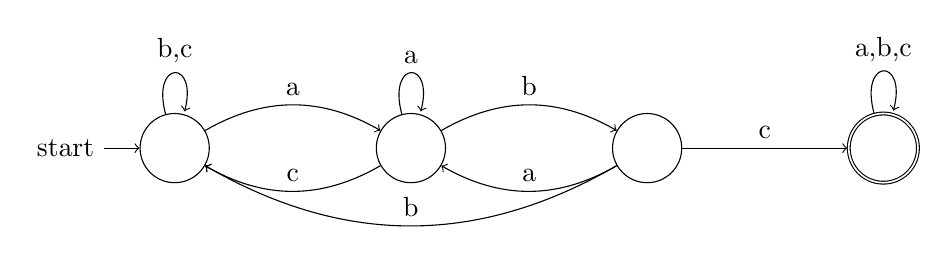
\begin{tikzpicture}[node distance = 3cm]

\node[state,initial] (1) {};
\node[state] (2) [right of = 1] {};
\node[state] (3) [right of = 2] {};
\node[state,accepting] (E) [right of = 3] {};

\path[->] (1) edge [bend left] node [above]  {a} (2)
    edge [loop above] node {b,c} ()
    (2) edge [bend left] node [above] {b} (3)
    edge [loop above] node {a} ()
    edge [bend left] node [above] {c} (1)
    (3) edge node [above] {c} (E)
    edge [bend left] node [above] {a} (2)
    edge [bend left] node [above] {b} (1)
    (E) edge [loop above] node {a,b,c} ();
\end{tikzpicture}

Dieser Automat akzeptiert alle Wörter über $\Sigma = \{a,b,c\}$, die abc enthalten. Dieser Automat beschreibt damit die formale Sprache aller Wörter, die abc enthalten.\\
Zur Darstellung von DFAs verwenden wir folgende graphische Notation:\\*
\begin{itemize}
\item Zustände: 
\begin{tikzpicture} \node[state] (1){}; \end{tikzpicture}
\item Startzustände 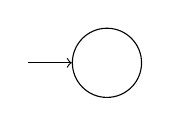
\begin{tikzpicture} \node[state] (1) at (0,0) {}; \draw [->] (-1,0) -- (1); \end{tikzpicture} [Hier im Script:] 
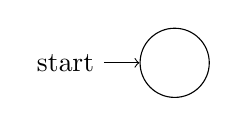
\begin{tikzpicture} \node[state,initial] (1){}; \end{tikzpicture}
\item Endzustände 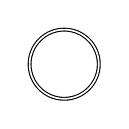
\begin{tikzpicture} \node[state,accepting] (E) {}; \end{tikzpicture}
\item Übergänge 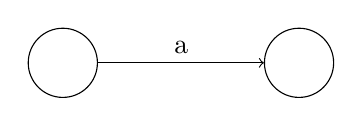
\begin{tikzpicture}[node distance = 3cm] \node[state] (2){};
\node[state] (3) [right of = 2] {}; \path[->] (2) edge node [above]  {a} (3); \end{tikzpicture}
\end{itemize}
Weiteres Beispiel: DFA, der alle Wörter akzeptiert, die auf aa enden.

\subparagraph{Defnition} Ein DFA ist ein Tupel $M=(Z,\Sigma,\delta,z_0,E)$
\begin{itemize}
\item $Z$: Menge der Zustände
\item $\Sigma$: Eingabealphabet
\item $\delta: Z \times \Sigma \to Z$: Überführungsfunktion
\item $z_0 \in Z$: Startzustand
\item $E \subseteq Z$: Endzustände
\end{itemize}

\subparagraph{Beispiel} Der DFA $M$, der alle Wörter akzeptiert, die abc enthalten, lässt sich formal beschreiben durch.\\
$M=(\{z_0,z_1,z_2,z_E\},\{a,b,c\},\delta,z_0,\{z_E\})$, wobei $\delta$ durch folgende Tabelle gegeben ist:
$\begin{array}{c|cccc}
\delta & z_0 & z_1 & z_2 & z_E\\ \hline
a & z_1 & z_1 & z_1 & z_E\\
b & z_0 & z_2 & z_0 & z_E\\
c & z_0 & z_0 & z_E & z_E\\
\end{array}$

\subparagraph{Definition} Sei $M=(Z,\Sigma,\delta,z_0,E)$ ein DFA.
\begin{itemize}
\item Die erweiterte Überführungsfunktion $\hat{\delta}: Z \times \Sigma^* \to Z$ von $M$ ist definiert durch:
\[ \hat\delta (z,w) = \left \{ \begin{array}{lcr}
z & \mbox{für} & w = \epsilon\\
\hat{\delta} (\delta(z,a),x) & \mbox{für} & w=ax \text{ mit } a \in \Sigma, x \in \Sigma^* \\
\end{array} \right.\]
\item Die von $M$ akzeptierte Sprache ist:
\[L(M) = \{ w \in \Sigma^* | \hat{\delta}(z_0,w) \in E\} \]
\end{itemize}

\subsubsection{Nichtdeterministische endliche Automaten (NFA)}
Ein NFA ist eine Verallgemeinerung eines DFA. Während ein DFA für jedes Paar aus Zustand und gelesenem Zeichen genau einen Folgezustand besitzt, besitzt der NFA beliebig viele Folgezustände.\\
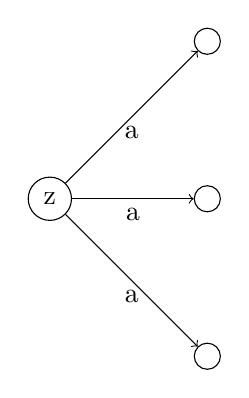
\begin{tikzpicture}
\node (z) at (0,0) [shape=circle,draw] {z};
\node (1) at (2,2) [shape=circle,draw] {};
\node (2) at (2,0) [shape=circle,draw] {};
\node (3) at (2,-2) [shape=circle,draw] {};
\draw [->] (z) -- (1)  node[midway,below] {a};
\draw [->] (z) -- (2)  node[midway,below] {a};
\draw [->] (z) -- (3)  node[midway,below] {a};
\end{tikzpicture}\\
Eine Möglichkeit, diesen Nichtdeterminismus zu verstehen, besteht darin, einen NFA als Modell zulässiger Zustandsfolgen zu betrachten.

Beispiel: NFA, der alle Wörter akzeptiert, die abc enthalten:\\
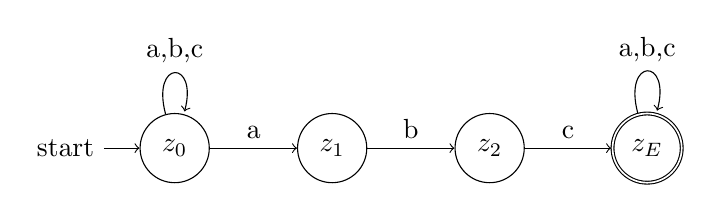
\begin{tikzpicture}[node distance = 2cm]
\node[state,initial] (z_0) {$z_0$};
\node[state] (z_1) [right of = z_0] {$z_1$};
\node[state] (z_2) [right of = z_1] {$z_2$};
\node[state,accepting] (z_E) [right of = z_2] {$z_E$};

\path[->] (z_0) edge node [above] {a} (z_1)
    edge [loop above] node {a,b,c} ()
    (z_1) edge node [above] {b} (z_2)
    (z_2) edge node [above] {c} (z_E)
    (z_E) edge [loop above] node {a,b,c} ();
\end{tikzpicture}\\
So wie eine Straßenkarte mögliche Wege beschreibt, beschreibt auch ein NFA mögliche Zustandsfolgen bei der Verarbeitung eines Wortes. Inbesondere "`weiß"' der NFA nicht, welchen Folgezustand er auswählen muss. Ein NFA lässt sich daher nicht unmittelbar als Programm implementieren.

Die von einem NFA $M$ akzeptierte Sprache $L(M)$ besteht aus allen Wörtern $w \in \Sigma^*$, für die $M$ einen Endzustand erreichen kann. Dabei müssen Kanten entsprechend der Zeichen der Eingabe durchlaufen werden.

\subparagraph{Beispiel (Fortsetzung)} Für die Eingabe $w=cbaab\underline{abc}c$ kann der NFA die Zustandsfolge $z_0,z_0,z_0,z_0,z_0,z_0,z_1,z_2,z_E,z_E$ durchlaufen. Da der letzte Zustand ein Endzustand ist, wird $w$ akzeptiert, d.h. $w \in L(M)$.\\
Für die Eingabe $abcabc$ gibt es zwei Zustandsfolgen, die zu $z_E$ führen $(z_0,z_0,z_0,z_0,z_1,z_2,z_E$ sowie $ z_0,z_1,z_2,z_E,z_E,z_E,z_E)$.\\ Daher gilt $abcabc \in L(M)$.

Für die Eingabe abba gibt es dagegen keine Zustandsfolge, mit der ein Endzustand erreicht werden kann. Daraus folgt $abba \notin L(M)$.

Eine alternative Möglichkeit, den Nichtdeterminismus eines NFA zu verstehen, besteht darin, einen NFA als Modell zu betrachten, das parallele Berechnungen beschreibt. Die durch einen NFA beschriebenen, möglichen Zustandsübergänge lassen sich dann durch einen Berechnungsbaum darstellen.:\\
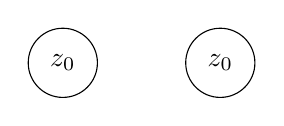
\begin{tikzpicture}[node distance = 2cm]
\node[state] (z_0_1) {$z_0$};
\node[state] (z_0_2) [right of = z_0_1] {$z_0$};
\end{tikzpicture}\\
Da es eine Folge von Berechnungen gibt, die zu einem Endzustand führt, wird die Eingabe akzeptiert.

Für einen NFA lässt sich die Überführungsfunktion definieren durch
\[ \delta: Z \times \Sigma \to \mathcal{P}(Z) \]
wobei $z' \in \delta(z,a)$ bedeutet: Wenn der NFA sich in Zustand $z$ befindet und das Zeichen $a$ erhält, dann kann er in den Zustand $z'$ wechseln.\\
Ferner besitzt ein NFA einen oder mehrere Startzustände.

Beispiel\\
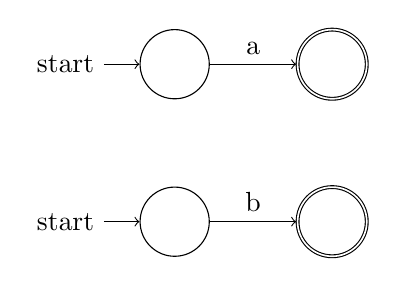
\begin{tikzpicture}[node distance = 2cm]
\node[state,initial] (1) {};
\node[state,accepting] (2) [right of = 1] {};
\node[state,initial] (3) [below of = 1] {};
\node[state,accepting] (4) [right of = 3] {};

\path[->] (1) edge node [above] {a} (2)
        (3) edge node [above] {b} (4);
\end{tikzpicture}\\
NFA, der die Sprache $\{a,b\}$ akzeptiert.

\paragraph{Umwandlung eines NFA in einen DFA}
Es gilt: Für jeden NFA gibt es einen DFA, der die gleiche Sprache erkennt. Idee zu Umwandlung: Wir vereinigen mögliche Folgezustände des NFA zu einem Zustand des DFA.\\
\begin{tikzpicture}[node distance = 2.3cm]
\node[state,initial] (1) {$z_0$};
\node[state,accepting] (2) [right of = 1] {$z_2$};
\node[state,initial] (3) [below of = 1] {$z_1$};
\node[state,accepting] (4) [right of = 3] {$z_3$};

\path[->] (1) edge node [above] {a} (2)
        edge node [above] {a} (4)
        (3) edge node [above] {a} (4);
\node [below of = 3] {NFA};
\node (arrow) [below right of = 2] {$\Rightarrow$};
\node (unvs) [right of = arrow] {};

\node[state,initial] (dfa1) [right of = unvs] {$\{z_0,z_1\}$};
\node[state] (dfa2) [right of = dfa1] {$\{z_2,z_3\}$};

\path[->] (dfa1) edge node [above] {a} (dfa2);

\node[below of = dfa1] {DFA};
\end{tikzpicture}\\
Falls es für einen Zustand $z$ und ein Zeichen $a$ keinen Folgezustand gibt (d.h. $\delta(z,a) = \varnothing$), führen wir einen Fehlerzustand ein, der nicht mehr verlassen werden kann.\\
\begin{tikzpicture}[node distance = 2 cm]
\node[state,initial] (a) {};
\node (b) [right of = a] {};

\path[->] (a) edge node [above] {c} (b);

\node (arrow) [right of = 2] {$\Rightarrow$};
\node (unvs) [right of = arrow] {};

\node[state,initial] (d) [right of = unvs] {};
\node (e) [right of = d] {};
\node[state] (f) [below of = d] {};
\path[->] (d) edge node [above] {c} (e)
        (d) edge node [right] {a,b} (f)
        (f) edge [loop left] node {a,b,c} ();

\end{tikzpicture}

Beispiel: Umwandlung des NFA\\
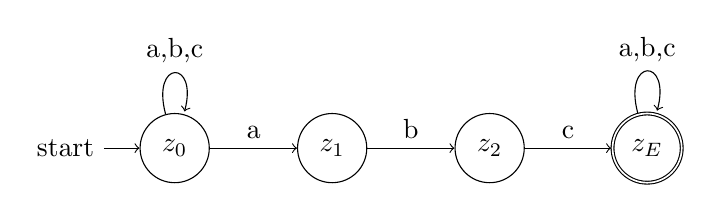
\begin{tikzpicture}[node distance = 2cm]
\node[state,initial] (z_0) {$z_0$};
\node[state] (z_1) [right of = z_0] {$z_1$};
\node[state] (z_2) [right of = z_1] {$z_2$};
\node[state,accepting] (z_E) [right of = z_2] {$z_E$};

\path[->] (z_0) edge node [above] {a} (z_1)
    edge [loop above] node {a,b,c} ()
    (z_1) edge node [above] {b} (z_2)
    (z_2) edge node [above] {c} (z_E)
    (z_E) edge [loop above] node {a,b,c} ();
\end{tikzpicture}\\
in einen DFA.\\
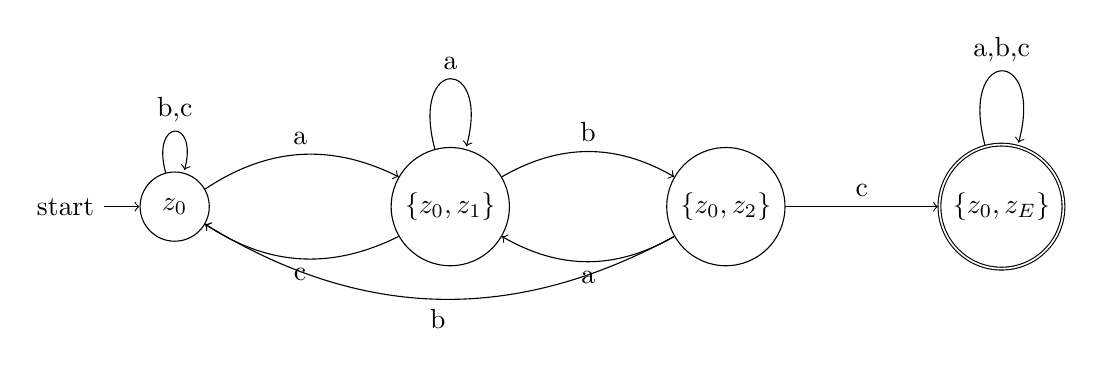
\begin{tikzpicture}[node distance = 3.5cm]
\node[state,initial] (z_0) {$z_0$};
\node[state] (z_01) [right of = z_0] {$\{z_0,z_1\}$};
\node[state] (z_02) [right of = z_01] {$\{z_0,z_2\}$};
\node[state,accepting] (z_0E) [right of = z_02] {$\{z_0,z_E\}$};

\path[->]   (z_0) edge [bend left] node [above] {a} (z_01)
             edge [loop above] node {b,c} ()
             (z_01) edge [bend left] node [below] {c} (z_0)
            edge [bend left] node [above] {b} (z_02)
            edge [loop above] node {a} ()
            (z_02) edge [bend left] node [below] {a} (z_01)
            edge [bend left] node [below] {b} (z_0)
            edge node [above] {c} (z_0E)
            (z_0E) edge [loop above] node {a,b,c} ()
                ;
\end{tikzpicture}\\
Der Zustand $\{z_0,z_E\}$ ist ein Endzustand, weil er einen Endzustand des NFA enthält.\\
Alle Zustände die von $\{z_0,z_E\}$ ausgehen, enthalten $z_E$ und sind damit ebenfalls Endzustände. Diese können vereinigt werden, ohne  die vom Automaten erkannte Sprache zu verändern.

Da die Potenzmenge $\mathcal{P}(Z)$ der Zustandsmenge des NFA $2^{\lvert z \rvert}$ Elemente enthält, kann der aus einem NFA umgewandelte DFA im schlimmsten Fall $2^{\lvert z \rvert}$ viele Zustände enthalten. Es ist möglich, dass sich darunter gleichwertige Zustände befinden, die zusammengefasst werden können.\\
Mit dem Algorithmus Minimalautomat kann aus einem DFA ein Automat erzeugt werden, der die gleiche Sprache erkennt und der minimal bezüglich der Anzahl der Zustände ist (Minimalautomat).\\
Je zwei Minimalautomaten unterscheiden sich höchstens in der Benennung der Zustände.
\subsection{Reguläre Ausdrücke}
\paragraph{Definition} Sei $\Sigma$ ein Alphabet. Ein regulärer Ausdruck $E$ über $\Sigma$ sowie die durch $E$  erzeugte Sprache $L(E)$ sind induktiv definiert:
\begin{enumerate}
\item $\varnothing$ ist ein regulärer Ausdruck $L(\varnothing) = \varnothing$.
\item Für jedes $a \in \Sigma \cup \{ \varepsilon \}$ ist $a$ ein regulärer Ausdruck und $L(a) = \{ a \}$.
\item Für reguläre Ausdrücke $E_1,E_2$ sind $(E_1 | E_2)$,
$(E_1E_2),(E_1^*)$ reguläre Ausdrücke und $L(E_1|E_2) = L(E_1) \cup L(E_2)$,\\
$L(E_1E_2) = L(E_1)L(E_2)$ (dabei ist $L(E_1)L(E_2) = \{ w_1w_2 | w_1 \in L(E_1), w_2 \in L(E_2)\}$)\\
$L(E_1^*) = (L(E_1))^*$
\end{enumerate}

Um Klammern zu sparen, legen wir folgende Regeln für die Priorität der Operatoren fest: Die höchste Priorität besitzt der Operator $*$, gefolgt von Konkatenation, gefolgt vom Operator $|$.

Beispiel:\\
$(a|b)^*$ ist ein regulärer Ausdruck und\\
$L((a|b)^*) = (L(a|b))^* = (L(a) \cup L(b))^* = ( \{a\} \cup \{b\})^* = \{a,b\}^*$.

\subparagraph{Satz} Für jeden regulären Ausdruck $E$ gibt es einen NFA $M$ mit $L(E) = L(M)$

Beweis: Wir induzieren über den Aufbau regulärer Ausdrücke:\\
Induktionsanfang:
\begin{itemize}
\item Für $E= \varnothing$ ist $M$ folgender NFA:
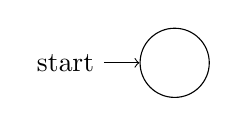
\begin{tikzpicture}
\node [state,initial] {};
\end{tikzpicture}
\item Für $E=a$ ist $M$ der NFA:
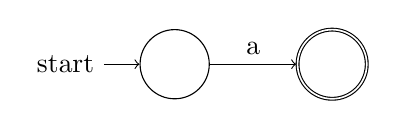
\begin{tikzpicture}[node distance = 2cm]
\node[state,initial] (z_1) {};
\node[state,accepting] (z_2) [right of = z_1] {};
\path[->] (z_1) edge node [above] {a} (z_2);
\end{tikzpicture}
\item Für $E= \varepsilon$ ist $M$ der NFA:
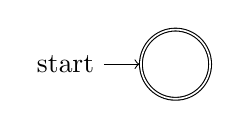
\begin{tikzpicture}
\node [state,initial,accepting] {};
\end{tikzpicture}
\end{itemize}

Induktionsschritt:\\
Seien $E_1,E_2$ reguläre Ausdrücke und nach Induktionsvorraussetzung $M_1',M_2'$ NFAs mit $L(E_1) = L(M_1'),L(E_2) = L(M_2')$. Ferner seien $M_1,M_2$ DFAs mit $L(M_1) = L(M_1'), L(M_2) = L(M_2')$
\begin{itemize}
\item $E1 | E_2$: Der NFA für $E_1 | E_2$ ist die "`Vereinigung"' von $M_1,M_2$, da ein NFA mehrere Startzustände haben darf.\\
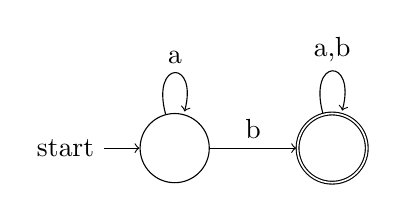
\begin{tikzpicture}[node distance = 2cm]
\node[state,initial] (z_1) {};
\node[state,accepting] (z_2) [right of = z_1] {};
\path[->] (z_1) edge node [above] {b} (z_2)
            edge [loop above] node {a} ()
            (z_2) edge [loop above] node {a,b} ();
\end{tikzpicture}
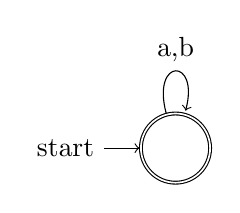
\begin{tikzpicture}
\node [state,initial,accepting] (z_1) {};
\path[->] (z_1) edge [loop above] node {a,b} ();
\end{tikzpicture}
\item $E_1E_2$: Skizze zur Idee:\\
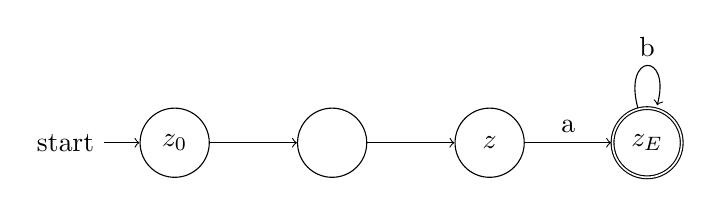
\begin{tikzpicture}[node distance = 2cm]
\node[state,initial] (z_0) {$z_0$};
\node[state] (z_1) [right of = z_0] {};
\node[state] (z_2) [right of = z_1] {$z$};
\node[state,accepting] (z_E) [right of = z_2] {$z_E$};

\path[->] (z_0) edge node [above] {} (z_1)
    (z_1) edge node [above] {} (z_2)
    (z_2) edge node [above] {a} (z_E)
    (z_E) edge [loop above] node {b} ();
\end{tikzpicture}\\
\begin{tikzpicture}[node distance = 2cm]
\node[state,initial] (z_0') {$z_0'$};
\node[state] (z_1') [right of = z_0] {};
\node[state,accepting] (z_E') [right of = z_1] {$z_E$};

\path[->] (z_0') edge node [above] {} (z_1')
    (z_1') edge node [above] {} (z_E');
\end{tikzpicture}\\
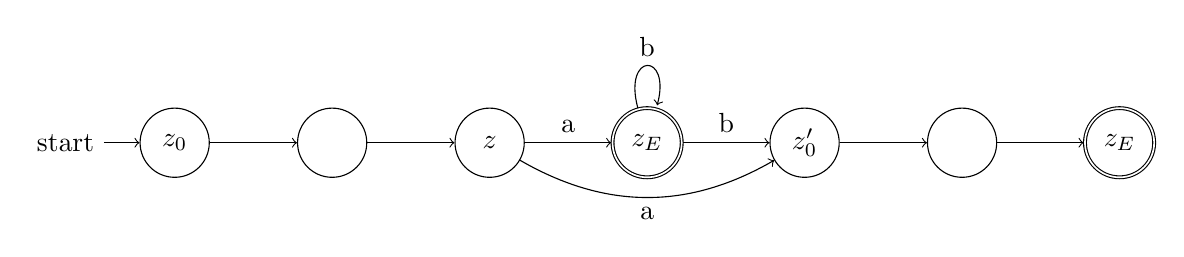
\begin{tikzpicture}[node distance = 2cm]
\node[state,initial] (z_0) {$z_0$};
\node[state] (z_1) [right of = z_0] {};
\node[state] (z_2) [right of = z_1] {$z$};
\node[state,accepting] (z_E) [right of = z_2] {$z_E$};

\path[->] (z_0) edge node [above] {} (z_1)
    (z_1) edge node [above] {} (z_2)
    (z_2) edge node [above] {a} (z_E)
    (z_E) edge [loop above] node {b} ();

\node[state] (z_0') [right of = z_E] {$z_0'$};
\node[state] (z_1') [right of = z_0'] {};
\node[state,accepting] (z_E') [right of = z_1'] {$z_E$};

\path[->] (z_0') edge node [above] {} (z_1')
    (z_1') edge node [above] {} (z_E')
    (z_E)  edge node [above] {b} (z_0')
    (z_2) edge [bend right] node [below] {a} (z_0');
\end{tikzpicture}
\item $E_1^*$ \\
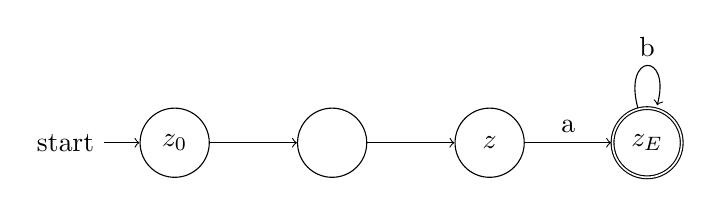
\begin{tikzpicture}[node distance = 2cm]
\node[state,initial] (z_0) {$z_0$};
\node[state] (z_1) [right of = z_0] {};
\node[state] (z_2) [right of = z_1] {$z$};
\node[state,accepting] (z_E) [right of = z_2] {$z_E$};

\path[->] (z_0) edge node [above] {} (z_1)
    (z_1) edge node [above] {} (z_2)
    (z_2) edge node [above] {a} (z_E)
    (z_E) edge [loop above] node {b} ();
\end{tikzpicture}\\
$\varepsilon \in L(E_1^*) \rightarrow$ 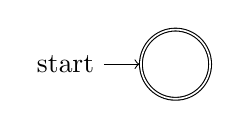
\begin{tikzpicture}
\node[state,initial,accepting] {};
\end{tikzpicture}\\
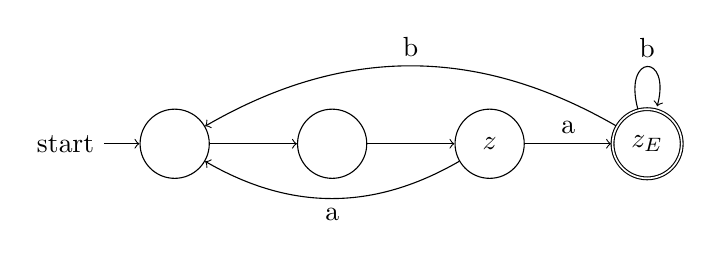
\begin{tikzpicture}[node distance = 2cm]
\node[state,initial] (z_0) {};
\node[state] (z_1) [right of = z_0] {};
\node[state] (z_2) [right of = z_1] {$z$};
\node[state,accepting] (z_E) [right of = z_2] {$z_E$};

\path[->] (z_0) edge node [above] {} (z_1)
    (z_1) edge node [above] {} (z_2)
    (z_2) edge node [above] {a} (z_E)
    (z_E) edge [loop above] node {b} ()
    (z_E) edge [bend right] node [above] {b} (z_0)
    (z_2) edge [bend left] node [below] {a} (z_0);
\end{tikzpicture}\\
\item $E^+ = EE^*$
\item $[E? = \varepsilon | E]$
\end{itemize}


\subparagraph{Satz} Für jeden NFA $M$ gibt es einen regulären Ausdruck $E$ mit $L(E) = L(M)$. Ohne Beweis.

Beispiel:\\
Sei $M$ der NFA 
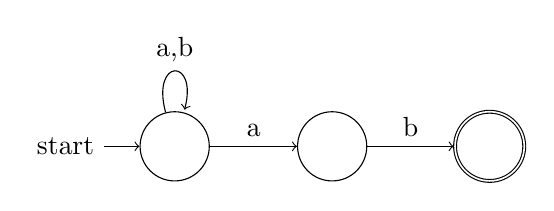
\begin{tikzpicture}[node distance = 2cm]
\node[state,initial] (z_0) {};
\node[state] (z_1) [right of = z_0] {};
\node[state,accepting] (z_2) [right of = z_1] {};

\path[->] (z_0) edge node [above] {a} (z_1)
    (z_1) edge node [above] {b} (z_2)
    (z_0) edge [loop above] node {a,b} ();
\end{tikzpicture}\\
Ein regulärer Ausdruck $E$ mit $L(E) = L(M) \text{ ist } (a|b)^* ab$.

\paragraph{Definition} Die Menge der regulären Sprachen ist die Menge der Sprachen, die von einem DFA erkannt werden.

Folgerung aus den bisher aufgeschriebenen Sätzen:\\
\begin{itemize}
\item Die NFAs erkennen genau die regulären Sprachen.
\item Die regulären Ausdrücke erzeugen genau die regulären Sprachen. 
\end{itemize}
Menge der regulären Sprachen = Sprachen, die von DFAs, NFAs oder von regulären Ausdrücken erkannt werden $\subset$ Menge aller Sprachen

\subparagraph{Lexer} Ein Lexer ist ein Werkzeug, das aus einem regulären Ausdruck einen DFA erzeugt, der die gleiche Sprache erkennt. Damit können Akzeptoren für Wörter aller Muster konstruiert werden.\\
Arbeitsweise eines Lexers:
regulärer Ausdruck $\rightarrow$ NFA $\rightarrow$ DFA

\subsection{Nichtreguläre Sprachen}
\paragraph{Satz} Die Sprache $L= \{a^nb^n | n \geq 0 \}$ ist nicht regulär.

Beweis:\\
Angenommen, $L$ sei regulär. Dann gibt es einen DFA $M$ mit $L(M) = L$. Nach dem Lesen von $a^n$ befindet sich $M$ in einem von $\lvert Z \rvert$ Zuständen. Da es mehr Präfixe $a^n$ als Zustände gibt, folgt aus dem Schubfachprinzip: Es gibt zwei verschiedene Wörter $a^{n_1},a^{n_2}$, so dass sich $M$ nach dem Lesen von $a^{n_1}$, bzw. $a^{n_2}$ im gleichen Zustand $z$ befindet.\\
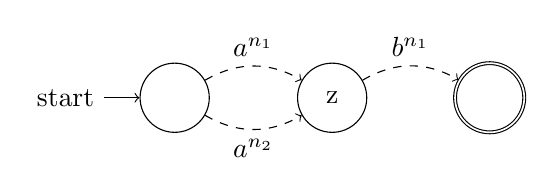
\begin{tikzpicture}[node distance = 2cm]
\node[state,initial] (z_0) {};
\node[state] (z_1) [right of = z_0] {z};
\node[state,accepting] (z_E) [right of = z_1] {};

\path[->,dashed] (z_0) edge [bend left] node [above] {$a^{n_1}$} (z_1)
    (z_0) edge [bend right] node [below] {$a^{n_2}$} (z_1)
    (z_1) edge [bend left] node [above] {$b^{n_1}$}(z_E);
\end{tikzpicture}\\
Da $M$ nach Annahme $a^{n_1} b^{n_1}$ akzeptiert, gelangt $M$ von $z$ aus, durch das Lesen von $b^{n_1}$, in einen Endzustand. Danach akzeptiert $M$ jedoch auch das Wort $a^{n_2}b^{_1}$, Widerspruch, da $n_1 \neq n_2$. 

\subsection{Kontextfreie Sprachen}
\subsubsection{Kellerautomaten (PDAs)}
Ein Kellerautomat (Pushdown Automaton, PDA) besitzt gegenüber einem NFA zwei zusätzliche Eigenschaften:
\begin{itemize}
\item Ein Kellerautomat kann den Zustand wechseln, ohne ein Eingabezeichen zu lesen ($\varepsilon$-Übergänge)
\item Ein Kellerautomat besitzt einen Stack (oder Keller bezeichnet), in dem er eine unbegrenzte Anzahl von Zeichen speichern kann.\\
Der Stack ist eine LIFO (last in, first out) Datenstruktur.
\end{itemize}
Ferner gibt es nur einen Startzustand, was wegen der $\varepsilon$-Übergänge keine Einschränkung ist.

Grapische Darstellung von PDAs: Wir erweitern die Darstellung von NFAs um Stackoperationen.\\
\begin{tikzpicture}[node distance = 3cm,stack/.style={rectangle split, rectangle split parts=#1,draw, anchor=center}]
\node[stack=4] (s1) [left of = z] {
\nodepart{one}$\gamma$
\nodepart{two}\vdots
\nodepart{three}\vdots
\nodepart{four}$\#$
}; \node [below of =s1] {Stack vorher};
\node[state] (z) {$z$}; \node[state] (z') [right of = z] {$z'$};
\path[->] (z) edge node [above] {$a,\gamma,\gamma'$} (z');
\node[stack=4] (s2) [right of = z'] {
\nodepart{one}$\gamma'$
\nodepart{two}\vdots
\nodepart{three}\vdots
\nodepart{four}$\#$
}; \node [below of =s2] {Stack nachher};

\end{tikzpicture}\\
Ein Übergang mit der Beschriftung $a,\gamma,\gamma'$ bedeutet:
\begin{itemize}
\item Der PDA liest das Zeichen $a$ der Eingabe, entfernt das oberste Stackzeichen $\gamma$ und schreibt $\gamma'$ auf den Stack.\\
\end{itemize}
Jedes der Zeichen $a,\gamma,\gamma'$ kann $\varepsilon$ sein. Für
\begin{itemize}
\item $a=\varepsilon$ kann der PDA diesen Übergang ausführen, ohne ein Zeichen der Eingabe zu lesen.
\item $\gamma = \varepsilon$ kann der PDA diesen Übergang ausführen, ohne das oberste Stackzeichen zu entfernen
\item $\gamma' = \varepsilon$ schreibt der PDA kein Zeichen auf den Stack
\end{itemize}
Damit ein PDA einen leeren Stack erkennen kann, wird das Ende des Stacks mit dem unterstem Stackzeichen $\#$ markiert. Zu Beginn jeder Rechnung enthält der Stack nur das Zeichen $\#$.\\
Ein PDA akzeptiert eine Eingabe, wenn er mit dieser einen Endzustand erreicht.

Beispiel: Ein PDA, der die Sprache $\{a^nb^n | n \geq 1\}$ akzeptiert. Für jedes gelesene $a$ wird dazu ein $a$ auf den Stack geschoben, für jedes gelesene $b$ ein $a$ vom Stack entfernt. Danach muss der Stack leer sein.

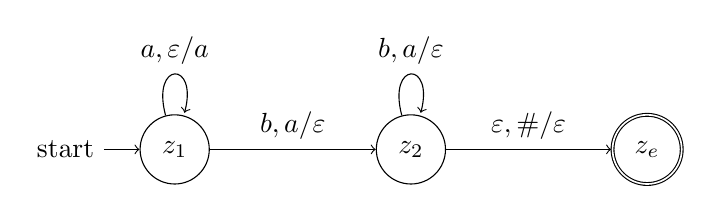
\begin{tikzpicture}[node distance = 3cm]
\node[state,initial] (z_0) {$z_1$};
\node[state] (z_1) [right of = z_0] {$z_2$};
\node[state,accepting] (z_e) [right of = z_1] {$z_e$};

\path[->] (z_0) edge node [above] {$b,a/\varepsilon$} (z_1)
                edge [loop above] node {$a,\varepsilon / a$} ()
                (z_1) edge node [above] {$\varepsilon,\# / \varepsilon$} (z_e)
                edge [loop above] node {$b,a/\varepsilon$}();
\end{tikzpicture}\\
Verhalten für die Eingabe $aaabbb$:
\begin{enumerate}
\item \begin{tikzpicture}[node distance = 3cm,stack/.style={rectangle split, rectangle split parts=#1,draw, anchor=center}]
\node[stack=1] (s1)  {
\nodepart{one}$\#$
}; \node [below of =s1] {$aaabbb$};
\end{tikzpicture}
\item \begin{tikzpicture}[node distance = 3cm,stack/.style={rectangle split, rectangle split parts=#1,draw, anchor=center}]
\node[stack=2] (s1) [left of = z] {
\nodepart{one}$a$
\nodepart{two}$\#$
}; \node [below of =s1] {aabbb};
\end{tikzpicture}
\item \begin{tikzpicture}[node distance = 3cm,stack/.style={rectangle split, rectangle split parts=#1,draw, anchor=center}]
\node[stack=3] (s1) [left of = z] {
\nodepart{one}$a$
\nodepart{two}$a$
\nodepart{three}$\#$
}; \node [below of =s1] {abbb};
\end{tikzpicture}
\item \begin{tikzpicture}[node distance = 3cm,stack/.style={rectangle split, rectangle split parts=#1,draw, anchor=center}]
\node[stack=4] (s1) [left of = z] {
\nodepart{one}$a$
\nodepart{two}$a$
\nodepart{three}$a$
\nodepart{four}$\#$
}; \node [below of =s1] {bbb};
\end{tikzpicture}
\item \begin{tikzpicture}[node distance = 3cm,stack/.style={rectangle split, rectangle split parts=#1,draw, anchor=center}]
\node[stack=3] (s1) [left of = z] {
\nodepart{one}$a$
\nodepart{two}$a$
\nodepart{three}$\#$
}; \node [below of =s1] {bb};
\end{tikzpicture}
\item \begin{tikzpicture}[node distance = 3cm,stack/.style={rectangle split, rectangle split parts=#1,draw, anchor=center}]
\node[stack=2] (s1) [left of = z] {
\nodepart{one}$a$
\nodepart{two}$\#$
}; \node [below of =s1] {b};
\end{tikzpicture}
\item \begin{tikzpicture}[node distance = 3cm,stack/.style={rectangle split, rectangle split parts=#1,draw, anchor=center}]
\node[stack=1] (s1) [left of = z] {
\nodepart{one}$\#$
}; \node [below of =s1] {};
\end{tikzpicture}
\item \begin{tikzpicture}[node distance = 3cm,stack/.style={rectangle split, rectangle split parts=#1,draw, anchor=center}]
\node[stack=1] (s1) [left of = z] {
\nodepart{one}$ $
}; \node [below of =s1] {};
\end{tikzpicture}
\end{enumerate}

Verhalten für $aab$
\begin{enumerate}
\item \begin{tikzpicture}[node distance = 3cm,stack/.style={rectangle split, rectangle split parts=#1,draw, anchor=center}]
\node[stack=1] (s1) [left of = z] {
\nodepart{one}$\#$
}; \node [below of =s1] {aab};
\end{tikzpicture}
\item \begin{tikzpicture}[node distance = 3cm,stack/.style={rectangle split, rectangle split parts=#1,draw, anchor=center}]
\node[stack=2] (s1) [left of = z] {
\nodepart{one}$a$
\nodepart{two}$\#$
}; \node [below of =s1] {ab};
\end{tikzpicture}
\item \begin{tikzpicture}[node distance = 3cm,stack/.style={rectangle split, rectangle split parts=#1,draw, anchor=center}]
\node[stack=3] (s1) [left of = z] {
\nodepart{one}$a$
\nodepart{two}$a$
\nodepart{three}$\#$
}; \node [below of =s1] {b};
\end{tikzpicture}
\item \begin{tikzpicture}[node distance = 3cm,stack/.style={rectangle split, rectangle split parts=#1,draw, anchor=center}]
\node[stack=2] (s1) [left of = z] {
\nodepart{one}$a$
\nodepart{two}$\#$
}; \node [below of =s1] {$\varepsilon$};
\end{tikzpicture}

\end{enumerate}
Sackgasse in $z_2$

Verhalten für $abb$
\begin{enumerate}
\item \begin{tikzpicture}[node distance = 3cm,stack/.style={rectangle split, rectangle split parts=#1,draw, anchor=center}]
\node[stack=1] (s1) [left of = z] {
\nodepart{one}$\#$
}; \node [below of =s1] {abb};
\end{tikzpicture}
\item \begin{tikzpicture}[node distance = 3cm,stack/.style={rectangle split, rectangle split parts=#1,draw, anchor=center}]
\node[stack=2] (s1) [left of = z] {
\nodepart{one}$a$
\nodepart{two}$\#$
}; \node [below of =s1] {bb};
\end{tikzpicture}
\item \begin{tikzpicture}[node distance = 3cm,stack/.style={rectangle split, rectangle split parts=#1,draw, anchor=center}]
\node[stack=1] (s1) [left of = z] {
\nodepart{one}$\#$
}; \node [below of =s1] {b};
\end{tikzpicture}
\end{enumerate}
$abb$ wird nicht akzeptiert, weil die Eingabe nicht bis zum Ende gelesen werden kann (ein $b$ ist noch übrig)\\

Im Folgenden erlauben wir, dass ein PDA mehrere Zeichen auf den Stack schreibt. Wir schreiben $a,\gamma/\gamma'_1 \dots \gamma'_n$, wenn der PDA zuerst $\gamma_n$ und zuletzt $\gamma_1$ auf den Stack schreibt.\\
\begin{tikzpicture}[node distance = 3cm,stack/.style={rectangle split, rectangle split parts=#1,draw, anchor=center}]
\node[stack=3] (s1) [left of = z] {
\nodepart{one}$\gamma$
\nodepart{two}\vdots
\nodepart{three}$\#$
}; \node [below of =s1] {Stack vorher};
\node[state] (z) {$z$}; \node[state] (z') [right of = z] {$z'$};
\path[->] (z) edge node [above] {$a,\gamma,\gamma'_1 \dots \gamma'_n$} (z');
\node[stack=5] (s2) [right of = z'] {
\nodepart{one}$\gamma'_1$
\nodepart{two}\vdots
\nodepart{three}$\gamma'_n$
\nodepart{four}\vdots
\nodepart{five}$\#$
}; \node [below of =s2] {Stack nachher};

\end{tikzpicture}\\

\subparagraph{Definition} Die von einem PDA $M$ akzeptierte Sprache $L(M)$ ist die Menge aller $w \in \Sigma^*$, für die gilt: Der PDA $M$ kann, ausgehend vom Startzustand und dem initialen Stackinhalt $\#$, durch das Lesen des Wortes $w$ einen Endzustand erreichen.

Bemerkung: Die deterministischen PDAs (DPDAs) sind weniger leistungsfähig als nichtdeterministische PDAs. Insbesondere lassen sich PDAs nicht umwandeln in DPDAs

\subsection{Kontextfreie Grammatiken}
Jede Grammatik besitzt ein Startsymbol und Ersetzungsregeln der Form linke Seite $\rightarrow$ rechte Seite. Beginnend mit dem Startsymbol können diese Regeln solange angewendet werden, bis keine Regel mehr anwendbar ist.\\
Bei einer kontextfreien Grammatik muss die linke Seite eine Variable sein.

Beispiel: Wir betrachten eine Grammatik, die aus den Variablen:\\
Satz, Nominalphrase, Verbalphrase, Artikel, Nomen, Verb\\
sowie den Terminalzeichen:\\
die, Katze, Maus, jagdt\\
besteht. Das Startsymbol ist Satz, die Regeln sind\\
Satz $\rightarrow$ Nominalphrase Verbalphrase\\
Nominalphrase $\rightarrow$ Artikel Nomen\\
Verb $\rightarrow$ jagt\\
Artikel $\rightarrow$ die\\
Nomen $\rightarrow$ Katze\\
Nomen $\rightarrow$ Maus\\
Verbalphrase $\rightarrow$ Verb\\
Verbalphrase $\rightarrow$ Verb Nominalphrase\\

Mögliche Ableitung:\\
Satz $\Rightarrow$ Nominalphrase Verbalphrase $\Rightarrow$ Artikel Nomen Verbalphrase $\Rightarrow$ die Nomen Verbalphrase $\Rightarrow$ die Katze Verbalphrase $\Rightarrow$ die Katze Verb Nominalphrase $\Rightarrow$  die Katze jagt Nominalphrase $\Rightarrow$ die Katze jagt Artikel Nomen $\Rightarrow$ die Katze jagt die Nomen $\Rightarrow$ die Katze jagt die Maus

Syntaxbaum dazu:\\

\begin{tikzpicture}
%level 1/.style={level distance=20mm,draw},
%\tikzstyle{level 1} = [level distance=20mm]
\tikzstyle{level 1} = [sibling distance = 50 mm]
\tikzstyle{level 2} = [sibling distance = 30 mm]
%\tikzstyle{level 3} = [sibling distance = 50 mm]
\node {Satz}
    child{node{NP}
        child{node{Artikel}
            child{node{die}}
        }
        child{node{Nomen}
            child{node{Katze}}
        }
    }
    child{node{VP}
        child{node{Verb}
            child{node{jagdt}}
        }
        child{node{NP}
            child{node{Artikel}
                child{node{die}}
            }
            child{node{Nomen}
                child{node{Maus}}
            }
        }
    }
;
\end{tikzpicture}

\paragraph{Definition} Eine kontextfreie Grammatik ist ein Tupel $G=(V,\Sigma,P,S)$, wobei gilt:
\begin{itemize}
\item $V$ ist die Menge der Variablen oder Nonterminalzeichen
\item $\Sigma$ ist das Alphabet mit $V \cap \Sigma = \varnothing$. Die Elemente aus $\Sigma$ heißen auch Terminalzeichen
\item $P$ ist die Menge der Regeln (oder Produktionen) der Form $u \to v$, wobei $u \in V, v \in (V \cup \Sigma)^*$.
\item $S \in V$ ist das Startsymbol
\end{itemize}

\subparagraph{Beispiel (Forts)} Die Grammatik lässt sich als Tupel $G= (V,\Sigma,P,S)$ darstellen, mit $V=\{\text{Satz},\text{Nominalphrase},\text{Verbalphrase},\text{Verb},\text{Artikel},\text{Nomen}\}$,\\
$\Sigma = \{$die,Katze,Maus,jagt$\}$,\\
$S=$ Satz und\\
$P$ wie oben.

Wir schreiben $x \Rightarrow y$, wenn sich aus $x \in (V \cup \Sigma)^*$ durch die Anwendung genau einer Regel $y \in (V \cup \Sigma)^*$ erzeugen lässt.

\subparagraph{Beispiel} Es gilt Satz $\Rightarrow$ Nominalphrase Verbalphrase $\Rightarrow$ Artikel Nomen Verbalphrase

\paragraph{Definition} Die Relation $\Rightarrow^*$ ist die reflexive und transitive Hülle der Relation $\Rightarrow$ (auf $(V\cup \Sigma)^*$)

\subparagraph{Beispiel} Es gilt
\begin{itemize}
\item Satz $\Rightarrow^*$ Satz
\item Satz $\Rightarrow^*$ Artikel, Nomen, Verbalphrase
\item Satz $\Rightarrow^*$ die Katze jagt die Maus
\end{itemize}

\subparagraph{Definition} Die von einer kontextfreien Grammatik $G$ erzeugte Sprache ist
\[L(G) = \{ w \in \Sigma^* | S \Rightarrow^* w \}\]
Wenn in einer kontextfreien Grammatik eine linke Seite durch verschiedene rechte Seiten ersetzt werden kann, verwenden wir das Zeichen $|$ (oder), um Alternativen anzugeben.

\subparagraph{Beispiel} Die Grammatik mit den Regeln
\begin{itemize}
\item $S \to \varepsilon$
\item $S \to SS$
\item$S \to [S]$ 
\end{itemize}
können wir damit kürzer darstellen durch\\
$S \to \varepsilon || SS | [S]$

\subparagraph{Beispiel} Durch die Grammatik mit den Regeln
\[S_N \to 0|1|\dots |9|0S_N|1S_N | \dots | 9S_N\] und dem Startsymbol $S_N$ können wir Zahlen aus $\mathbb{N}_0$ darstellen. Die Zahl 120 lässt sich ableiten durch $S_N \Rightarrow 1S_N \Rightarrow 12 S_N \Rightarrow 120$. Diese Regeln verwenden wir in einer weiteren Grammatik, um arithmetische Ausdrücke zu erzeugen.
\begin{itemize}
\item Die Operatoren $+,-,*,/$ sind binär, weshalb vor und nach jedem Operator ein arithmetischer Ausdruck stehen muss.
\item Auf jede öffnende Klammer muss eine schließende Klammer folgen.

\end{itemize}

Damit erhalten wir die Grammatik mit den Regeln.
\[ S_E \rightarrow S_N | (S_E) | S_E \text{ Op } S_E \]
und dem Startsymbol $S_E$.\\
Der Ausdruck $2 *(3+4)$ lässt sich ableiten durch\\
$S_E \Rightarrow S_E * S_E \Rightarrow S_N * S_E \Rightarrow 2 * S_E \Rightarrow 2*(S_E) \Rightarrow 2*(S_E + S_E) \Rightarrow 2*(S_N + S_E) \Rightarrow 2*(S_N + S_n) \Rightarrow 2*(3+ S_N) \Rightarrow 2*(3+4)$

\subparagraph{Definition} Eine Sprache $L$ heißt kontextfrei, wenn es eine kontextfreie Grammatik $G$ gibt, mit $L(G) = L$.

\subsubsection{PDAs und kontextfreie Grammatiken}
\subparagraph{Satz} Kellerautomaten (PDAs) akzeptieren genau die kontextfreien Sprachen.

Beweis:
\begin{enumerate}
\item Für jeden PDA $M$ gibt es eine kontextfreie Grammatik $G$ mit $L(M) = L(G)$. Ohne Beweis.
\item Für jede kontextfreie Grammatik $G$ gibt es einen PDA $M$ mit $L(M) = L(G)$
\end{enumerate}
Idee: $M$ simuliert auf seinen Stack Ableitungen aus der Grammatik $G$.

Wir konstruieren einen PDA $M$ mit drei Zuständen wie folgt:
\begin{itemize}
\item Zuerst schreibt $M$ das Startsymbol $S$ auf den Stack und wechselt in einen weiteren Zustand.
\end{itemize}
In diesem Zustand unterscheiden wir drei Fälle:\\
Das oberste Stackzeichen ist
\begin{itemize}
\item eine Variable $A$. Wenn es eine Regel $A \rightarrow \gamma$ in $G$ gibt, kann $M$ das oberste Stackzeichen $A$ durch $\gamma$ ersetzen.
\item ein Zeichen $a \in \Sigma $, das mit den nächsten Zeichen der Eingabe übereinstimmt. Dann wird $a$ vom Stack entfernt.
\item $\#$. Dann geht $M$ in den Endzustand über.
\end{itemize}

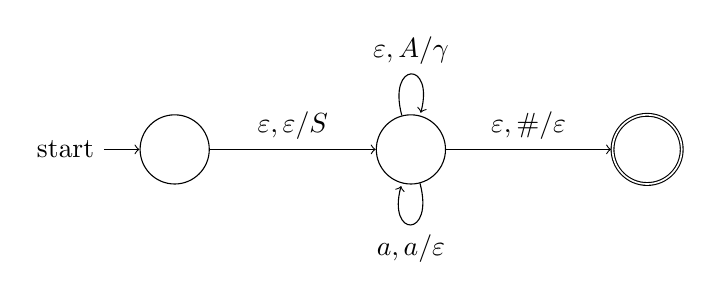
\begin{tikzpicture}[node distance = 3cm]
\node[state,initial] (z_0) {};
\node[state] (z_1) [right of = z_0] {};
\node[state,accepting] (z_2) [right of = z_1] {};

\path[->] (z_0) edge node [above] {$\varepsilon,\varepsilon / S$} (z_1)
    (z_1) edge [loop above] node {$\varepsilon,A / \gamma$} ()
    (z_1) edge node [above] {$\varepsilon,\# / \varepsilon$} (z_2)
    (z_1) edge [loop below] node {$a,a / \varepsilon$} ();
\end{tikzpicture}

\subparagraph{Beispiel} Für die Sprache $L = \{ a^n b^n | n \geq 0 \}$ konstruieren wir einen PDA $M$ mit $L(M) = L$. $L$ wird erzeugt von der Grammatik mit den Regeln $S \rightarrow aSb | \varepsilon$.\\
Aus obigen Beweis erhalten wir den PDA.\\
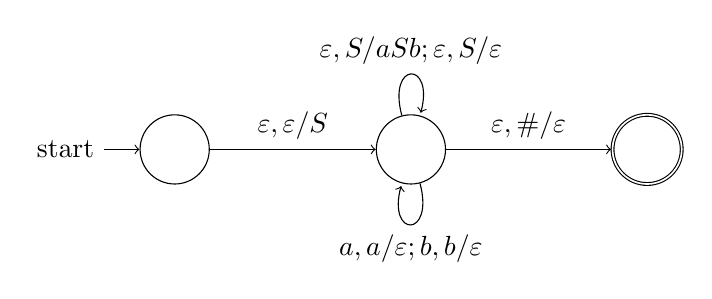
\begin{tikzpicture}[node distance = 3cm]
\node[state,initial] (z_0) {};
\node[state] (z_1) [right of = z_0] {};
\node[state,accepting] (z_2) [right of = z_1] {};

\path[->] (z_0) edge node [above] {$\varepsilon,\varepsilon / S$} (z_1)
    (z_1) edge [loop above] node {$\varepsilon,S / aSb ; \varepsilon,S / \varepsilon$} ()
    (z_1) edge node [above] {$\varepsilon,\# / \varepsilon$} (z_2)
    (z_1) edge [loop below] node {$a,a / \varepsilon ; b,b / \varepsilon$} ();
\end{tikzpicture}

Verhalten für $aabb$:
\begin{enumerate}
\item 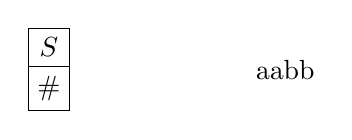
\begin{tikzpicture}[node distance = 3cm,stack/.style={rectangle split, rectangle split parts=#1,draw, anchor=center}]
\node[stack=2] (s1) {
\nodepart{one}$S$
\nodepart{two}$\#$
}; \node [right of =s1] {aabb};
\end{tikzpicture}
\item 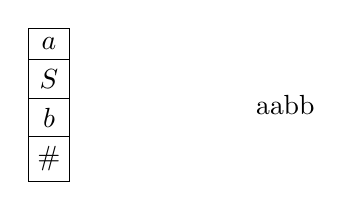
\begin{tikzpicture}[node distance = 3cm,stack/.style={rectangle split, rectangle split parts=#1,draw, anchor=center}]
\node[stack=4] (s1) {
\nodepart{one}$a$
\nodepart{two}$S$
\nodepart{three}$b$
\nodepart{four}$\#$
}; \node [right of =s1] {aabb};
\end{tikzpicture}
\item \begin{tikzpicture}[node distance = 3cm,stack/.style={rectangle split, rectangle split parts=#1,draw, anchor=center}]
\node[stack=3] (s1) {
\nodepart{one}$S$
\nodepart{two}$b$
\nodepart{three}$\#$
}; \node [right of =s1] {abb}; \end{tikzpicture}
\item \begin{tikzpicture}[node distance = 3cm,stack/.style={rectangle split, rectangle split parts=#1,draw, anchor=center}]
\node[stack=5] (s1) {
\nodepart{one}$a$
\nodepart{two}$S$
\nodepart{three}$b$
\nodepart{four}$b$
\nodepart{five}$\#$
}; \node [right of =s1] {abb};\end{tikzpicture}
\item \begin{tikzpicture}[node distance = 3cm,stack/.style={rectangle split, rectangle split parts=#1,draw, anchor=center}]
\node[stack=4] (s1) {
\nodepart{one}$S$
\nodepart{two}$b$
\nodepart{three}$b$
\nodepart{four}$\#$
}; \node [right of =s1] {bb};\end{tikzpicture}
\end{enumerate}

\paragraph{Syntaxanalyse}
Arbeitsweise eines Compilers\\
\begin{tikzpicture}[node distance = 1cm]
\node (Ausd) {$\text{if}(x<0 || y < 0 ) \{ \dots \} \text{else if} \dots$};
\node (Lexer) [below of = Ausd] {Lexer};
\node (Gep) [below of = Lexer] {$
\begin{array}{|c|c|c|c|c|c|c|c|c|c|c|c|c|c|c|c|}\hline
\text{if} & ( & \text{ID} & < & \text{NUM} & \text{OR} & \text{ID} & < & \text{NUM} & ) & \{ & \dots & \} & \text{ELSE} & \text{IF} & \dots \\ \hline
\end{array}$};
\node (Parser) [below of = Gep] {Parser};
\node (Syntaxbaum) [below of = Parser] {Syntaxbaum};
\node (Code-Erzeuger) [below of = Syntaxbaum] {Code-Erzeuger};

\path[->] (Ausd) edge (Lexer)
        (Lexer) edge (Gep)
        (Gep) edge (Parser)
        (Parser) edge (Syntaxbaum)
        (Syntaxbaum) edge (Code-Erzeuger);
\end{tikzpicture}

Parser lassen sich in zwei Klassen unterteilen:

\paragraph{Top-Down-Parser} Ein Top-Down-Parser erzeugt einen Syntaxbaum von oben nach unten.\\
Ein Top-Down-Parser arbeitet wie das Verfahren aus dem Beweis zur Umwandlung einer kontextfreien Grammatik in einen PDA. Ein Top-Down-Parser lässt sich durch rekursive Prozeduren implementieren, von denen jede einer Regel der Grammatik entspricht. Der Callstack übernimmt die Funktion des Stack des PDA. Wir erlauben dem Parser, die $k$ nächsten Zeichen der Eingabe zu sehen (lookahead von $k$), um davon abhängig eine Regel auszuwählen.

Beim Verarbeiten der Eingabe baut ein Top-Down-Parser implizit den Syntaxbaum von oben nach unten auf.\\
Beispiel: Parser für $\{ a^nb^n | n \geq 0 \}$, Eingabe $aabb$\\
\begin{tikzpicture}
\node {$S()$}
    child {node {match$('a')$}}
    child {node {$S()$}
        child {node {match$('a')$}}
        child {node {$S()$}
            child {node {return true}}
        }
        child {node {match$('b')$}}
    }
    child {node {match$('b')$}}
;
\end{tikzpicture}\\
Der Callgraph besitzt die gleiche Struktur wie der Syntaxbaum.

Ein Parser, der durch rekursive Funktionen einen Syntaxbaum von oben nach unten aufbaut, heißt Recursive Descent Parser.

\paragraph{Mehrdeutigkeit}
\subparagraph{Definition}
Eine Grammatik $G$ heißt mehrdeutig, wenn es ein $w\in L(G)$ gibt, für das zwei Ableitungsbäume existieren.

Beispiel: Die Grammatik für arithmetische Ausdrücke mit den Regeln
\[ E \rightarrow E +E | E-E | E*E | E / E | (E) | x | y | z \]
ist mehrdeutig, denn der Ausdruck $x+y*z$ besitzt zwei Ableitungsbäume.\\
\begin{tikzpicture}
\node {$E$}
    child {node {$E$}
        child {node {$x$}}
        }
    child {node {$+$}}
    child {node {$E$}
        child {node {$E$}
            child {node {$y$}}
            }
        child {node {$*$}}
        child {node {$E$}
            child {node {$z$}}
            }
    };
\end{tikzpicture}
\begin{tikzpicture}
\node {$E$}
    child {node {$E$}
        child {node {$E$}
            child{node {$x$}}
        }
        child {node {$+$}}
        child {node {$E$}
            child {node {$y$}}
        }
    }
    child {node {$*$}}
    child {node {$E$}
        child {node {$z$}}
    };
\end{tikzpicture}

Auch wenn wir nur den Operator "`-"' betrachten, ist die Grammatik mehrdeutig, denn der Ausdruck $x-y-z$ besitzt die Ableitungsbäume:\\*
\begin{tikzpicture}
\node (first) {$E$}
    child {node{$E$}
        child {node {$E$}
            child{node (leftbottom) {$x$}}
        }
        child {node{$-$}}
        child {node{$E$}
            child {node{$y$}}
        }
    }
    child {node{$-$}}
    child {node{$E$}
        child{node{$z$}}
    }
;
\node [below  of = leftbottom] {$(x-y)-z$};
\end{tikzpicture}
\begin{tikzpicture}
\node {$E$}
    child{node{$E$}
        child{node{$x$}}
    }
    child {node{$-$}}
    child{node{$E$}
        child{node{$E$}
            child{node (leftbottom) {$y$}}
        }
        child {node{$-$}}
        child{node{$E$}
            child{node{$z$}}
        }
    }
;
\node [below of = leftbottom] {$x-(y-z) \Rightarrow x-y+z$};
\end{tikzpicture}



Mit obiger Grammatik gibt es mehrere Probleme
\begin{itemize}
\item Sie berücksichtigt nicht die Priorität der Operatoren (Punkt vor Strich)
\item Sie berücksichtigt nicht die Assoziativität der Operatoren
\end{itemize}

Um das Problem der Priorität zu lösen, definieren wir eine Grammatik, bei der sich Operatoren niedriger Priorität oben im Ableitungsbaum und Operatoren höherer Priorität weiter unten im Ableitungsbaum befinden müssen.\\
Wir führen dazu eine Variable $T$ (Term) ein, aus der Produkte abgeleitet werden können. Für die Produktionen aus $E$ gibt es folgende Möglichkeiten:
\begin{equation} \label{1}
E \rightarrow E-T | E+T | T
\end{equation}
oder
\begin{equation}\label{2}
E \rightarrow T -E | T+E | T
\end{equation}
Sowohl mit (\ref{1}) als auch (\ref{2}) ist gewährleistet, dass die Operatoren $+,-$ oben im Ableitungsbaum vorkommen.\\
Mit (\ref{1}) ist folgende Ableitung möglich.

\begin{tikzpicture}
\node {$E$}
    child{node{$E$}
        child{node{$E$}
            child{node{$T$}}
        }
        child{node{$-$}}
        child{node{$T$}}
    }
    child{node {$-$}}
    child{node{$T$}}
;
\end{tikzpicture} entspricht $(T-T)-T$, d.h. $-$ ist links-assoziativ.\\
Mit (\ref{2}) ist folgende Ableitung möglich\\
\begin{tikzpicture}
\node{$E$}
    child{node{$T$}}
    child{node{$-$}}
    child{node{$E$}
        child{node{$T$}}
        child{node{$-$}}
        child{node{$E$}
            child{node{$T$}}
                    }
    }
    
;
\end{tikzpicture}
entspricht $T-(T-T)$, d.h. $-$ wäre rechtsassoziativ.

Nur Grammatik (\ref{1}) berücksichtigt sowohl die Priorität als auch die Assoziativität der Operatoren $+,-$ in korrekter Weise. Entsprechend definieren wir Regeln für $T$ und erhalten:
\[ E \rightarrow E-T | E+T | T\]
\[ T \rightarrow T*F | T / F | F\]
\[ F \rightarrow (E) | x |y|z\]

Diese Grammatik ist eindeutig und berücksichtigt Priorität und Assoziativität der Operatoren.\\
Der eindeutige Ableitungsbaum für $x+y*z$ ist\\
\begin{tikzpicture}
\node {$E$}
    child{node{$E$}
        child{node{$T$}
            child{node{$F$}
                child{node{$x$}}
            }
        }
    }
    child{node{$+$}}
    child{node{$T$}
        child{node{$T$}
            child{node{$F$}
                child{node{$y$}}
            }
        }
        child{node{$*$}}
        child{node{$F$}
            child{node{$z$}}
        }
    }
;
\end{tikzpicture}

Der Ableitungsbaum für $x-y-z$ ist\\
\begin{tikzpicture}
\node{$E$}
    child{node{$E$}
    child{node{$E$}
        child{node{$T$}
            child{node{$F$}
                child{node{$x$}}
            }
        }
        child{node{$-$}}
        child{node{$T$}
            child{node{$F$}
                child{node{$y$}}
            }
        }
    }
    child{node{$-$}}
    child{node{$T$}
        child{node{$F$}
            child{node{$z$}}
        }
    }
}
;
\end{tikzpicture}

\paragraph{Bottom-up Parser} Ein Buttom-up Parser baut einen Ableitungsbaum von unten nach oben auf. Diese lassen sich effizient realisieren durch LR-Parser. Ein LR-Parser liest die Eingabe von links nach rechts und führt in jedem Schritt eine von vier möglichen Aktionen aus:
\begin{itemize}
\item Shift: Das nächste Zeichen der Eingabe wird auf den Stack geschoben.
\item Reduce: Ein oder mehrere Symbole an der Spitze des Stacks entsprechen der rechten Seite $\gamma$ einer Regel $A \rightarrow \gamma$ und werden durch $A$ ersetzt.
\item Accept: Die Eingabe wurde verarbeitet und der Stack enthält nur das Startsymbol.
\item Error: Ein Syntaxfehler wird gemeldet.
\end{itemize}
Um zu entscheiden, welche Aktion (Shift oder Reduce) auszuführen ist, verwendet der Parser eine Parsetabelle.

Beispiel Mit der eindeutigen Grammatik von oben und der Eingabe $x+y+z$ führt ein LR-Parser folgende Aktionen aus:\\
\begin{tabular}{r|c|c}
Stack\\
bottom  top & Restliche Eingabe & Aktion\\ \hline
 & $x+y*z$ & $s$ \\
 $x$ & $+y*z$ & $r$\\
 $F$ & $+y*z$ & $r$\\
 $T$ & $+y*z$ & $r$\\
 $E$ & $+y*z$ & $s$\\
 $E+$ & $y*z$ & $s$\\
 $E+y$ & $*z$ & $r$\\
 $E+F$ & $*z$ & $r$\\
 $E+T$ & $*z$ & $s$\\
 $E+T*$ & $z$ & $s$\\
 $E+T*z$ & & $r$\\
 $E+T*F$ & & $r$\\
 $E+T$ & & $r$\\
 $E$ & & $accept$\\
\end{tabular}\\
Die vom Parser konstruierte Rechtsableitung lässt sich aus den ersten beiden Spalten von unten nach oben ablesen.
Ebenso kann der Parser den Wert des Ausdrucks berechnen, wenn Zwischenwerte in den Symbolen gespeichert werden.

Zur Konstruktion von LR-Parsern werden Tools wie Yacc,Bison, \textsc{Cup} verwendet.

Wenn wir die eindeutige Grammatik für arithmetische Ausdrücke in einen Recursive Descent Parser überführen wollen, stellen sich zwei Probleme:
\begin{itemize}
\item Es ist nicht erkennbar, welche Regel ausgewählt werden soll
\item Die Regel $E \rightarrow E+T$ ist linksrekursiv. Diese führt zu einer endlosen Rekursion.
\end{itemize}
Wir brauchen daher eine andere Grammatik.

Mögliche Lösung:
\[ E \rightarrow T+E | T-E | T \]
Dann sind die Operatoren jedoch rechtsassoziativ, also würde die Grammatik falsche Ergebnisse berechnen.

\paragraph{EBNF}(Erweiterte Backus-Naur-Form)\\*
Wir betrachten Ableitungen aus $E$:\\*
\[ E \Rightarrow E + T \Rightarrow E+T+T \Rightarrow \dots \Rightarrow T + \dots + T \]
In EBNF lässt sich dies darstellen durch
\[ E \rightarrow T \{ +T \} \text{ (alternat. Notation: } E \rightarrow T (+T)^* \text{ )} \]
Dabei bedeutet $\{x\}$: beliebig viele Vorkommen von x.

Die Grammatik für arithmetische Ausdrücke lässt sich in EBNF wie folgt darstellen:
\[E \rightarrow T \{ + T | -T\}\]
\[T \rightarrow F \{*F |  /F\} \]
\[F \rightarrow (E) | \text{Num} \]
\[\text{Num} \rightarrow Z \{Z\} \]
\[Z \rightarrow 0| \dots |9\]
Aus der Darstellung in EBNF lassen sich Syntaxdiagramme ableiten:\\
$E:$\\ %TODO 2014-05-20T13:44
$F:$\\

Problem: Aus der Darstellung in EBNF oder den Syntaxdiagrammen ist nicht ersichtlich, welche Assoziativität die Operatoren haben. Ohne weitere Annahmen (z.B: alle Operatoren linksassoziativ) ist diese Grammatikbeschreibung nicht eindeutig.

Wir wollen nun eine eindeutige Grammatik für Ausdrücke in Infix-Notation konstruieren, die eindeutig und nicht linksrekursiv ist.
\[E \rightarrow T E_{\text{Tail}}\]
\[E_{\text{Tail}} \rightarrow \varepsilon  | +E | -E\]
\[T \rightarrow F T_{\text{Tail}} \]
\[T_{\text{Tail}} \rightarrow \varepsilon | * T | /T\]
\[F \rightarrow (E) | \text{Num} \]
\[\text{Num} \rightarrow Z \text{Num}_{\text{Tail}} \]
\[\text{Num}_{\text{Tail}} \rightarrow \varepsilon | \text{Num} \]
\[Z \rightarrow 0 | \dots | 9 \]

Beispiel: Ableitung des Ausdrucks $3+2*4$\\*
\begin{tikzpicture} 
\tikzstyle{level 1} = [sibling distance = 50 mm]
\tikzstyle{level 2} = [sibling distance = 30 mm]
\node{$E$}
    child{node{$T$}
        child{node{$F$}
            child{node{Num}
                child{node{$Z$}
                    child{node{$3$}}
                }
                child{node{$\text{Num}_{\text{Tail}}$}
                    child{node{$\varepsilon$}}
                }
            }
        }
        child{node{$T_{\text{Tail}}$}
            child{node{$\varepsilon$}}
        }
    }
    child{node{$E_{\text{Tail}}$}
        child{node{$+$}}
        child{node{$E$}
            child{node{$T$}
                child{node{$F$}
                    child{node{Num}
                        child{node{$Z$}
                            child{node{$2$}}
                        }
                        child{node{$\text{Num}_{\text{Tail}}$}
                            child{node{$\varepsilon$}}
                        }
                    }
                }
                child{node{$T_{\text{Tail}}$}
                    child{node{$*$}}
                    child{node{$T$}
                        child{node{$F$}
                            child{node{Num}
                                child{node{$Z$}
                                    child{node{$4$}}
                                }
                                child{node{$\text{Num}_{\text{Tail}}$}
                                    child{node{$\varepsilon$}}
                                }
                            }
                        }
                        child{node{$T_{\text{Tail}}$}
                            child{node{$\varepsilon$}}
                        }
                    }
                }
            }
        }
    }
;
\end{tikzpicture}

\subsubsection{0L-Systeme}
Eine Turtle besitzt eine Position in der Ebene und eine Orientierung. Zeichenbefehle sind:
\begin{itemize}
\item forward(l)
\item left($\alpha$) bzw. right($\alpha$). Dreht die Turtle
\end{itemize}
Ein 0L-System besteht, wie eine kontextfreie Grammatik, aus Variablen, Terminalzeichen und Regeln: In jedem Ableitungsschritt müssen jedoch alle Variablen ersetzt werden durch eine Regel.

Beispiel: Koch-Kurve\\
Variablen: $F$\\
Terminalzeichen: $+,-$\\
Regeln: $F \rightarrow F + F -- F +F$

\section{Teil 2}
\subsection{Berechenbarkeit und Komplexität}
\subsubsection{Entscheidbarkeit}
Ist es möglich, durch einen Algorithmus festzustellen, ob ein Programm $P$ eine bestimmte Eigenschaft besitzt.\\
\begin{tikzpicture}[node distance = 5cm]
\node[rectangle] (P) {Programm $P$};
\node[rectangle,draw] (EV) [right of = P] {Entscheidungsverfahren};
\node[rectangle] (jn) [right of = EV] {ja/nein};

\path[->] (P) edge (EV)
        (EV) edge (jn);
\end{tikzpicture}\\*
Eigenschaften können sein:
\begin{itemize}
\item Das Programm $P$ stürzt nicht ab
\item Das Programm $P$ liefert immer eine Antwort
\item Das Programm $P$ terminiert immer
\end{itemize}
\subparagraph{Beispiel}
\begin{lstlisting}[numbers=left, tabsize=4, style=customc,mathescape]
for (k >= 3)
    for (x,y,z := 1 to k)
        for (n = 3 to k)
            if (x^n + y^n = z^n) stop
\end{lstlisting}
Dieses Programm sucht nach einen Gegenbeispiel zu der von Fermat aufgestellten Behauptung (Fermats letzter Satz), dass die Gleichung $x^n + y^n = z^n$ keine Lösung in $x,y,z \in \mathbb{N}$ für $n \geq 3$ besitzt. Dies war über Jahrhunderte ein ungelöstes Problem. Offenbar gilt: Das Programm hält genau dann wenn Fermats letzter Satz falsch ist.

Weiteres Problem: Ist es entscheidbar ob ein Programm $P$ "`Hello World"' ausgibt?\\
\begin{tikzpicture}[node distance = 5cm]
\node[rectangle] (P) {Programm $P$};
\node[rectangle,draw] (EV) [right of = P] {Entscheidungsverfahren};
\node[rectangle] (jn) [right of = EV] {ja, gibt HW aus/ nein};

\path[->] (P) edge (EV)
        (EV) edge (jn);
\end{tikzpicture}\\
Man betrachte dazu das Programm
\begin{lstlisting}[numbers=left, tabsize=4, style=customc]
void P() {
    fermat();
    printf("Hello World");
}
\end{lstlisting}
Da $P()$ genau dann "`Hello World"' ausgibt, wenn fermat() terminiert, ist dieses Problem mindestens so schwierig wie das Halteproblem.

Um Berechenbarkeit zu untersuchen, verwenden wir Programme auf einen abstrakten mit unbegrenzten Speicher und Variablen, die beliebig große Werte annehmen können, als Berechnungsmodell.

\subparagraph{Definition} Eine Sprache $L$ heißt entscheidbar, wenn es ein Programm $P_L$ gibt, mit der Eigenschaft
\begin{itemize}
\item Für die Eingabe $w \in L$ liefert $P_L$ true
\item Für die Eingabe $w \notin L$ liefert $P_L$ false
\end{itemize}
In Pseudocode
\begin{lstlisting}[numbers=left, tabsize=4, style=customc,mathescape]
boolean $P_L$ ($w$) {
    if ($w \in L$) return true;
    else return false;
}
\end{lstlisting}

Übung: Zeigen Sie, dass folgende Sprachen entscheidbar sind:
\begin{itemize}
\item $\varnothing$
\item $\Sigma^*$
\item Die Sprache aller Palindrome
\item $\{ (M,w) | M$ ist ein DFA mit $w \in L(M))\}$
\item $\{M | M$ ist ein DFA mit $L(M) = \Sigma^*\}$
\end{itemize}
\begin{tikzpicture} [node distance = 2cm]
\node[state,initial] (z_1) {$z_1$};
\node[state,accepting] (z_2) [right of = z_1] {$z_2$};

\path[->] (z_1) edge node [above] {$a$} (z_2)
                edge [loop above] node {$b$} ()
               (z_2) edge [loop above] node {$a,b$}();
\end{tikzpicture}\\
$\begin{array}{c|cc}
\delta & z_1 & z_2 \\ \hline
a & z_2 & z_2 \\
b & z_1 & z_2 \\
\end{array}$\\
$(\{z_1,z_2\},z_1,\{\{z_2,z_2\},\{z_1,z_2\}\}, \{z_2\})$

Die Srpache $\varnothing$ ist entscheidbar durch das Programm
\begin{lstlisting}[numbers=left, tabsize=4, style=customc,mathescape]
boolean $P_\varnothing$ ($w$) {
    return false;
}
\end{lstlisting}
$\Sigma^*$ ist entscheidbar durch das Programm
\begin{lstlisting}[numbers=left, tabsize=4, style=customc,mathescape]
boolean $P_{\Sigma^*}$ ($w$) {
    return true;
}
\end{lstlisting}
Die Sprache aller Palindrome ist entscheidbar durch
\begin{lstlisting}[numbers=left, tabsize=4, style=customc,mathescape]
boolean $P_{\text{Palindrom}}$ ($w$) {
    for (i=1 to length(w) /2 )
        if (w[i] $\neq$ w[length(w) -i])
            return false;
    return true;
}
\end{lstlisting}

Die Sprache in $\{ (M,w) | M$ ist ein DFA mit $w \in L(M))\}$ ist entscheidbar durch das Programm
\begin{lstlisting}[numbers=left, tabsize=4, style=customc,mathescape]
boolean $P_d$ (DFA $M$,word $w$) {
    return simmulate(M,w);
}
\end{lstlisting}
wobei simmulate(M,w) den DFA $M$ für die Eingabe $w$ simuliert. Dies ist möglich (vgl. HA).

$\{M | M$ ist ein DFA mit $L(M) = \Sigma^*\}$ ist entscheidbar durch
\begin{lstlisting}[numbers=left, tabsize=4, style=customc,mathescape]
boolean $P_e$ (DFA $M$) {
    return Minimalautomat(M) == $M_{\Sigma^*}$;
}
\end{lstlisting}
wobei $M_{\Sigma^*}$ der DFA \begin{tikzpicture} \node[state,initial,accepting] (z_1) {};
\path[->] (z_1) edge [loop above] node {} ();
\end{tikzpicture}

HA: Ist $\{(M_1,M_2) |L(M_1) = L(M_2) \}$ entscheidbar


\subparagraph{Das Halteproblem}
Das Halteproblem ist formal die Sprache
\[ H = \{ (P,w) | \text{Das Programm } P \text{ hält für die Eingabe } w \} \]
Die Frage, ob ein Programm $P$, gegeben als Text, für eine Eingabe $w$ hält, ist damit gleichwertig zu der Frage, ob $(P,w) \in H$ gilt.\\
Um zu zeigen, dass $H$ unentscheidbar ist, zeigen wir zunächst:
\subparagraph{Satz} Das spezielle Halteproblem
\[ K = \{ P | \text{Das Programm } P \text{ hält für die Eingabe } P \}\]
ist unentscheidbar.

Beweis: Angenommen, $K$ ist entscheidbar durch ein Programm $P_K$.\\
Daraus konstruieren wir ein Programm $P_K^*$, das $P_K$ als Unterprogramm benutzt und das 
\begin{itemize}
\item in eine Endlosschleife übergeht, wenn $P_K$ true liefert
\item hält, wenn $P_K$ false liefert\\
\begin{tikzpicture}[node distance = 5cm]
\node[rectangle,draw] (P_K) {$P_K$};
\node[rectangle] (0) [left of = P_K] {};
\node[circle,draw] (halt) [above right of = P_K] {};
\node[rectangle] (loop1) [right of = P_K] {};
\node[rectangle] (loop) [below right of = loop1] {};
\node[rectangle] (P_K^*) [below left of = P_K] {$P_K^*$};
\draw (-4,-4) rectangle (4,4);
\path[->] (0) edge  node [above] {$P$} (P_K)
        (P_K) edge  node [above] {true} (halt)
        edge node [below] {false} (loop);
\end{tikzpicture}
\end{itemize}
Nach Konstruktion gilt damit:
\begin{itemize}
\item Für die Eingabe $P$ hält $P_K^*$ genau dann, wenn $P_K$ false liefert. Da $P_K$ nach Annahme die Sprache $K$ entscheid, bedeutet dies:
\item Für die Eingabe $P$ hält $P_K^*$ genau dann, wenn $P$ nicht hält. Da dies für beliebige $P$ gilt, können wir $P=P_K^*$ wählen. Damit folgt:
\item Für die Eingabe $P_K^*$ hält $P_K^*$ genau dann, wenn $P_K^*$ nicht hält und damit ein Widerspruch.
\end{itemize}

\subparagraph{Weitere unentscheidbare Probleme}
Mit der Untentscheidbarkeit des speziellen Halteproblems können wir die Unentscheidbarkeit weiterer Probleme zeigen. Um zu zeigen, dass eine Sprache $B$ nicht entscheidbar ist, verwenden wir eine unentscheidbare Sprache $A$. Wir zeigen, dass mit der Annahme, $B$ sei entscheidbar, ein Entscheidungsverfahren für $A$ konstruieren lässt. Aus diesem Widerspruch folgt die Unentscheidbarkeit von $B$.

\subparagraph{Satz} $H$ ist nicht entscheidbar.

Beweis: Angenommen $H$ sei entscheidbar. Dann können wir folgendes Programm konstruieren, das das angenommene Entescheidungsverfahren $P_H$ für $H$ als Unterprogramm verwendet:\\
\begin{lstlisting}[numbers=left, tabsize=4, style=customc,mathescape]
boolean $P_K$ (Programm $P$) {
    return $P_H(P,P)$
}
\end{lstlisting}

Damit wäre aber $P_K$ ein Entscheidungsverfahren für $K$, Widerspruch.\\
Damit folgt, dass auch die Programmverifikation unentscheidbar ist.

\subparagraph{Satz} \[\text{Verify } = \{ (P,S) | \text{Das Programm erfüllt die Spezifikation } S \} \]
ist nicht entscheidbar.

Beweis: Angenommen Verify ist entscheidbar durch ein Programm $P_{\text{verify}}$. Dann können wir das Programm konstruieren.
\begin{lstlisting}[numbers=left, tabsize=4, style=customc,mathescape]
boolean $P_H$(Programm $P$, Input $w$) {
    return $P_{\text{verify}}$($P$, $P \text{ hält für die Eingabe } w$)
}
\end{lstlisting}
das dann ein Entscheidungsverfahren für $H$ ist, Widerspruch.

\subparagraph{Satz} \[H_\varepsilon = \{ P | P \text{ hält für die Eingabe } \varepsilon \}\] ist nicht entscheidbar.

Beweis: Sei wieder angenommen, $H_\varepsilon$ sei entscheidbar, durch ein Programm $P_{H_\varepsilon}$. 
\begin{lstlisting}[numbers=left, tabsize=4, style=customc,mathescape]
boolean $P_H$(Programm $P$, Input $w$){
    void F(){
        P(w)
    }
    return $P_{H_\varepsilon}$ (F)
}
\end{lstlisting}
Dann ist $P_H$ aber ein Entscheidungsverfahren für das Halteproblem, denn $(P,w) \in H  \Leftrightarrow P$ hält für $w \Leftrightarrow F$, hält für $\varepsilon \Leftrightarrow F \in H_\varepsilon$ und damit Widerspruch.

\subparagraph{Weitere unentscheidbare Probleme} Fast alle Probleme im Zusammenhang mit Programmverifikation, z.B.
\begin{itemize}
\item $\{ P |P$ verursacht eine Division durch $0$ für eine Eingabe $\}$
\item $\{P|P$ verursacht einen Buffer-Overflow für eine Eingabe $\}$
\item $\{ (P_1,P_2) |P_1$ verhält sich wie $P_2 \}$
\end{itemize}

\subparagraph{Mathematische Probleme}
\begin{itemize}
\item $\{F |$ Die durch die Formel $F$ ausgedrückte Funktion ist $x \to 0 \}$
\item $\{ S | S$ ist eine wahre mathematische Aussage $\}$
\end{itemize}

\subsection{Komplexitätstheorie}
Wir beschränken uns nun auf entscheidbare Probleme und betrachten den Aufwand zur Lösung dieser Probleme:

\subsubsection{Die Klassen P und NP}
Für die $\mathcal{O}$-Notation gelten folgende Rechenregeln:
\begin{itemize}
\item $\mathcal{O} (f+g) = \mathcal{O} (f) + \mathcal{O} (g)$
\item $\mathcal{O} (f+g) = \mathcal{O} (\max{(f,g)})$
\item $\mathcal{O} (c\cdot f) = \mathcal{O} (f)$ für eine Konstante $c >0$
\item $\mathcal{O} (f \cdot g) = \mathcal{O} (f) \cdot \mathcal{O} (g)$
\end{itemize}
Bei der Laufzeitmessung von Algorithmen verwenden wir das uniforme Kostenmaß, bei dem die Laufzeit aller Einzeloperationen (wie Zuweisung, Vergleich, Addition) in $\mathcal{O} (1)$ liegt.

\subparagraph{Definition} Die Komplexitätklasse \textsc{P} ist definiert durch 
\[ \textsc{P} = \bigcup\limits_{k \geq 1} \, \{ L | L \text{ ist entscheidbar durch ein Programm mit Laufzeit in } \mathcal{O} (n^k) \} \]
wobei $n$ die Länge der Eingabe ist.

Beispiele: Folgende Sprachen liegen in \textsc{P}:
\begin{itemize}
\item Die Sprache aller Palindrome: Das Programm
\begin{lstlisting}[numbers=left, tabsize=4, style=customc,mathescape]
boolean P (String w ) {
    return w= reverse(w)
}
\end{lstlisting}
stellt für alle $w \in \Sigma^*$ in der Zeit $\mathcal{O} (\lvert w \rvert)$ fest, ob $w$ ein Palindrom ist. Dabei seien reverse sowie "`="' Funktionen mit linearer Laufzeit.
\item Die Sprache $\{ a^nb^n | n \geq 0 \}$, da diese durch einen Rekursive Descent Parser in Zeit $\mathcal{O} (n)$ entschieden werden kann.
\item Jede kontextfreie Sprache. Es gibt einen Algorithmus der jede kontextfreie Sprache in Zeit $\mathcal{O} (n^3)$ entscheidet.
\item \textsc{Pfad} $= \{ (G,n_1,n_2) | G$ ist ein Graph, in dem es einen Pfad von $n_1$ nach $n_2$ gibt $\}$, wobei $G$ durch eine Adjazenzliste gegeben sei. Denn da die Adjazenzliste eines Graphen $G= (V,E)$ mindestens $\lvert V \rvert + \lvert E \rvert$ Elemente enthält, gilt für die Länge $n$ der Eingabe $n \geq \lvert V \rvert + \lvert E \rvert$. Ein Entscheidungsverfahren für \textsc{Pfad} ist eine in $n_1$ gestartete Breitensuche mit Ziel $n_2$. Deren Laufzeit liegt in $\mathcal{O} (\lvert V \rvert + \lvert E \rvert)$. Aus $\lvert V \rvert + \lvert E \rvert \leq n$ folgt:\\*
$\mathcal{O} (\lvert V \rvert + \lvert E \rvert) \subseteq \mathcal{O} (n)$. Damit liegt die Laufzeit in des Entscheidungsverfahren in $\mathcal{O} (n)$, woraus \textsc{Pfad} $\in P$ folgt.

\end{itemize}

Ferner gibt es Sprachen, die nicht offensichtlich in $P$ liegen.\\
Wichtiges Beispiel:
\[ \textsc{SAT} = \{ F | F \text{ ist eine erfüllbare Formel der Aussagenlogik} \}\]
z.B. gilt $(x \vee y ) \wedge z \in \textsc{ SAT}, \quad \neg x \wedge x \notin \textsc{SAT} $

Um für eine Formel $F$ zu prüfen, ob $F \in \textsc{SAT}$ gilt, können wir alle $2^n$ Belegungen erzeugen und jeweils den Wahrheitswert berechnen ($n$ sei die Anzahl der Variablen in $F$).\\
Die Laufzeit dieses Entscheidungsverfahren liegt in $\mathcal{O} (2^n \cdot f(n))$, wobei $f(n)$ die Zeit ist, um den Wahrheitswert zu berechnen.

Wir können jedoch in polynomieller Zeit verifizieren, dass $F \in \textsc{SAT}$ gilt, wenn eine erfüllende Belegung $c_F$ für $F$ bekannt ist. Denn dazu muss das Entscheidungsverfahren lediglich den  Wahrheitswert von $F$ unter der Belegung $c_F$ berechnen, was in der Zeit $\mathcal{O} (\lvert F \rvert )$ möglich ist.

\subparagraph{Definition} Die Komplexitätsklasse \textsc{NP} ist definiert durch 
\[ \textsc{NP} = \bigcup\limits_{k \geq 1} \,\{ L | L \text{ ist verifizierbar in Zeit } \mathcal{O} (n^k) \} \]
wobei $n$ die Länge der Eingabe ist.

Beispiel: Es gilt $\textsc{SAT} \in \textsc{NP}$, da mit einer erfüllenden Belegung für $F$ in Zeit $\mathcal{O} ( \lvert F \rvert )$ verifiziert werden kann, ob $F \in \textsc{SAT}$ gilt.

Es gilt $\textsc{P} \subseteq \textsc{NP}$, denn für jede Sprache $L \in \textsc{P}$ gibt es ein Entscheidungsverfahren mit einer Laufzeit in $\mathcal{O} (n^k)$. Dies ist ebenfalls ein Verifizierungsverfahren das kein Zertifikat verwendet.

Unbekannt ist, ob $\textsc{P} = \textsc{NP}$ gilt.\\
Die Klasse \textsc{P} wird betrachtet als Klasse der effizient lösbaren Probleme. Gründe dazu:
\begin{itemize}
\item Die meisten Probleme in \textsc{P} lassen sich in Zeit $\mathcal{O} (n^k)$ mit einem kleinen $k$ lösen. Diese Probleme sind damit auch praktisch lösbar.
\end{itemize}

\subsubsection{NP-vollständige Probleme}
Die \textsc{NP}-vollständigen Probleme sind eine Klasse von Problemen in \textsc{NP}, für die keine effizienten Entscheidungsverfahren bekannt sind. Alle bekannten Verfahren besitzen exponentielle Laufzeit.\\
Die \textsc{NP}-vollständigen Probleme sind mindestens so schwierig wie jedes andere Problem in \textsc{NP}.\\
Es gilt: Wenn ein effizientes Entscheidungsverfahren für ein \textsc{NP}-vollständiges Problem gefunden wird, dann ist für jedes Problem in \textsc{NP} ein effizientes Entscheidungsverfahren bekannt. Genauer:

\subparagraph{Satz} Es gilt \textsc{P = NP} genau dann, wenn es ein \textsc{NP}-vollständiges Problem $L$ mit $L \in \textsc{P}$ gibt.

Man vermutet, dass $\textsc{P} \neq \textsc{NP}$ gilt, weil bisher kein \textsc{NP}-vollständiges Problem in \textsc{P} gefunden wurde.\\
Situation für $\textsc{P} \neq \textsc{NP}$:\\*
\begin{tikzpicture}[scale = 0.75]
\draw (5,0) circle [radius = 1] node {P};
\draw (10,0) circle [radius = 1] node {NP-v.};
\draw (7.5,-2) circle [radius = 5] node {NP};
\draw (7.5,-2) circle [radius = 6]; \node at (7.5,-7.3) {Entscheidbare Probleme};
\draw (7.5,-2) circle [radius = 7]; \node at (7.5,-8.5) {Alle Sprachen};
\end{tikzpicture}

\subparagraph{Satz} Das Erfüllbarkeitsproblem der Aussagenlogik
\[ \text{SAT} = \{ F | F \text{ ist eine erfüllbare Formel der Aussagenlogik} \}
\]
ist \textsc{NP}-vollständig.

Bemerkung: Das schnellste bekannte Verfahren für SAT hat die Laufzeit $\mathcal{O}(1,308^n \cdot p(n))$, wobei $p$ ein Polynom ist.

Anwendungen:
\begin{itemize}
\item Autokonfiguration: Die bestellbaren Konfigurationen kann man durch Regeln in Form von aussagenlogischen Formelen beschreiben, z.B:\\
Sportfahrwerk $\rightarrow$ Leichtm $\wedge$ (Motor 2.0 $\vee$ Motor 2.5 $\vee$ Motor 3.0)\\
Alle derartigen Formel werden mit $\wedge$ verknüpft zu einer Formel $F_1$. Die Wünsche des Kunden lassen sich als Formel $F_2$ beschreiben. Die Kundenwünsche sind erfüllbar, wenn $F_1 \wedge F_2$ erfüllbar ist.
\item Vereinfachen von Schaltkreisen\\
Angenommen, es ist ein Referenzentwurf für einen Schaltkreis vorhanden. Dieser Entwurf soll nun vereinfacht werden (weniger Gatter), um die Herstellungskosten zu senken. Um zu prüfen, ob dieser Schaltkreis gleichwertig zum Referenzentwurf ist, wird der Referenzentwurf durch eine Formel $F_R$ der Aussagenlogik, der vereinfachte Schaltkreis durch eine Formel $F_S$.\\
Dann muss $F_R \leftrightarrow F_S$ eine Tautologie sein. Dies ist gleichwertig damit, dass $\neg (F_R \leftrightarrow F_S)$ unerfüllbar ist. D.h., beide Schaltkreise sind gleichwertig genau dann, wenn $\neq (F_R \leftrightarrow F_S) \notin \text{SAT}$.
\end{itemize}

\subparagraph{Satz} Das Problem $\textsc{Hamilton-Kreis} = \{ G |$ Der Graph $G$ besitzt einen Hamiltonkreis $\}$ ist NP-vollständig.

Verallgemeinerung davon: Traveling Salesman Problem (TSP). Gegeben $n$ Städte und Verbindungen zwischen diesen Städten, gesucht ist eine kürzeste Rundreise durch alle Städte.

\subparagraph{Satz} Das Problem $TSP = \{(M,k)|M$ ist eine Entfernungsmatrix und es gibt eine Rundreise der Länge $\leq k \}$ ist \textsc{NP}-vollständig.

Bemerkung: Das Problem, eine kürzeste Rundreise zu berechnen, ist mindestens so schwierig wie obiges Entscheidungsproblem.\\
Anwendungen:
\begin{itemize}
\item Platine bohren: Um die Bohrzeit für eine Platine zu minimieren, muss ein TSP- für die Bohrlöcher gelöst werden.
\item Auf einer Fertigungsstraße sollen Produkte $P_1,\dots,P_n$ hergestellt werden. Dazu muss die Fertigungsstraße jeweils umgerüstet werden. Sei $d_{ij}$ der Zeitaufwand, um eine Fertigungsstraße die Produkt $i$ herstellt, für Produkt $j$ umzurüsten.\\
Um eine Reihenfolge festzulegen, die die Summe der Rüstzeiten minimiert, muss ein TSP für die Matrix $(d_{ij})$ gelöst werden
\end{itemize}

Weiteres, ähnliches Problem: Kürzester Hamiltonpfad\\
Dieses Problem ist ebenfalls \textsc{NP}-vollständig.

\subparagraph{Anwendung} DNA-Sequenzierung\\
Eine DNA-Sequenz ist ein Wort über dem Alphabet $\{A,C,G,T\}$.\\
Um eine DNA zu sequenzieren, wird diese in kleine Bruchstücke geschnitten, diese sequenziert, und aus diesen Bruchstücken die ursprüngliche Sequenz rekonstruiert.

Ansatz dazu: Kürzeste gemeinsame Obersequenz (Shortest Common Supersequence) bestimmen, d.h. eine kürzeste Sequenz finden, die alle Bruchstücke als Teilwort enthält.\\
Dazu wird anhand der Überlappung zweier Bruchstücke ein Abstand berechnet und damit ein Short Common Superstring bzw. kürzester Hamiltonpfad-Pfad-Problem gelöst.

\subparagraph{Beispiel} Ursprüngliche Sequenz: $ATGCAA$\\*
Bruchstücke: $ATG,CAA,GCA,TGC$

Algorithmen für TSP:
\begin{itemize}
\item Nearest Neighbor Greedy Algorithmus:\\
Starte in einem beliebigen Knoten\\
Solange noch nicht alle Knoten besucht wurden:
Wähle einen nächsten unbesuchten Nachbarn des aktuellen Knoten aus und verlängere den aktuellen Pfad

Greedy-Algorithmen wählen in jeden Schritt eine lokal optimale Teillösung aus. Greedy-Algorithmen können optimal sein. Für das TSP ist der Greedy-Algorithmus nicht optimal, er kann beliebig schlechte Lösungen liefern.

\item Es gibt einen Algorithmus, der eine optimale Lösung liefert, mit Laufzeit in $\mathcal{O} (n^2 2^n)$, wobei $n= \lvert V \rvert$.

\item Approximation: Wir versuchen, einen Rundweg zu finden, dessen Länge etwa so groß ist, wie die kürzeste Länge.\\
Das metrische TSP ist ein TSP, bei dem der Abstand $d_{ij}$ zweier Knoten eine Metrik ist. Für das metrische TSP gibt es einen Approximationsalgorithmus mit Laufzeit in $\mathcal{O} (n^2 \log{n})$, der eine Lösung liefert, die eine Länge $\leq 2\cdot \text{optimale Länge}$ besitzt.
\end{itemize}

\subparagraph{Das Rucksackproblem} Ein Rucksack der Größe $S>0$ soll mit einer Auswahl von Gegenständen $1,\dots,n$ der Größe $s_1,\dots,s_n > 0$ maximal bepackt werden. Gesucht ist also eine Menge $C \subseteq \{1,\dots,n\}$ mit 
\[ \sum\limits_{k \in C} s_k \leq S\] und
\[ \sum\limits_{k \in C} s_k \text{ maximal}\]

Anwendungen:
\begin{itemize}
\item CD mit mp3 optimal befüllen
\item Budget maximal verbrauchen
\end{itemize}
Das Rucksackproblem ist \textsc{NP}-vollständig.

Algorithmus für Rücksack:\\
Sei $r(k,s)$ die maximale Füllmenge eines Rucksackes der Größe $s, \; 0 \leq s \leq S$, der mit einer Auswahl von Gegenständen $1,\dots,k$ bepackt ist. Gesucht ist $r(n,S)$. Wir berechnen $r(k,s)$ für $1 \leq k \leq n, 0 \leq s \leq S$ mit Hilfe einer %%

Feststellung: Wenn für alle $0 \leq l \leq s, r(k-1,l)$ bereits bekannt ist, lässt sich daraus $r(k,s)$ berechnen:
\begin{itemize}
\item Wenn der Gegenstand $k$ nicht eingepackt wird, gilt
\[ r(k,s) = (k-1,s) \]
\item Wenn der Gegenstand $k$ eingepackt wird, gilt
\[ r(k,s) = r(k-1,s-s_k) + s_k \]
\end{itemize}
Daraus ergibt sich
\[ r(k,s) = \left \{ \begin{array}{lcr} 0 & \text{für} & k= 0 \\ r(k-1,s) & \text{für} & s < s_k\\ \max{(r(k-1,s),r(k-1,s-s_k)+s_k)} & & \text{sonst}\\ \end{array} \right. \]
Laufzeit: $\mathcal{O}(nS)$.\\*
Dies ist kein Widerspruch dazu, dass Rucksack \textsc{NP}-vollständig ist, denn die Länge der Eingabe ist $\log_2{S} + \sum\limits_{k=1}^{n} \log_2{s_k}$\\
$S= 2^{\log_2{S}}$









\end{document}